\documentclass{sigchi}

% Load basic packages
\usepackage{balance}  % to better equalize the last page
\usepackage{graphics} % for EPS, load graphicx instead
\usepackage{times}    % comment if you want LaTeX's default font
\usepackage{url}      % llt: nicely formatted URLs
\usepackage{caption}
\usepackage{subcaption}
\usepackage{float}
\usepackage{pdfpages}
\usepackage{booktabs}
\usepackage{multirow}

\toappear{
Paper submitted for evaluation in the Pervasive Computing Course, Autumn 2014. The IT University of Copenhagen.\\ Copyright remains with the authors.
}

% llt: Define a global style for URLs, rather that the default one
\makeatletter
\def\url@leostyle{%
  \@ifundefined{selectfont}{\def\UrlFont{\sf}}{\def\UrlFont{\small\bf\ttfamily}}}
\makeatother
\urlstyle{leo}


% To make various LaTeX processors do the right thing with page size.
\def\pprw{8.5in}
\def\pprh{11in}
\special{papersize=\pprw,\pprh}
\setlength{\paperwidth}{\pprw}
\setlength{\paperheight}{\pprh}
\setlength{\pdfpagewidth}{\pprw}
\setlength{\pdfpageheight}{\pprh}

% Make sure hyperref comes last of your loaded packages,
% to give it a fighting chance of not being over-written,
% since its job is to redefine many LaTeX commands.
\usepackage[pdftex]{hyperref}
\hypersetup{
pdftitle={Deciding presence and interruptibility automatically using only a laptop},
pdfauthor={Kristian S. M. Andersen, Anders Bech Mellson and Mads Daniel Christensen},
pdfkeywords={spce, gse, presence, awareness},
bookmarksnumbered,
pdfstartview={FitH},
colorlinks,
citecolor=black,
filecolor=black,
linkcolor=black,
urlcolor=black,
breaklinks=true,
}

% create a shortcut to typeset table headings
\newcommand\tabhead[1]{\small\textbf{#1}}

% Double lined table cells
\newcommand{\specialcell}[2][c]{%
  \begin{tabular}[#1]{@{}c@{}}#2\end{tabular}}

% End of preamble. Here it comes the document.
\begin{document}

\title{Deciding presence and interruptibility automatically using only a laptop}
\numberofauthors{3}
\author{
  \alignauthor Anders Bech Mellson\\
    \email{anbh@itu.dk}\\
  \alignauthor Kristian S. M. Andersen\\
    \email{ksma@itu.dk}\\
  \alignauthor Mads D. Christensen\\
    \email{mdch@itu.dk}\\
}

\maketitle

\begin{abstract}
When a person needs the attention of another person, it is essential to find the right time to start the interaction.
It is natural to glance at another person and estimate how occupied they are. With this estimation, we can judge if our interruption is socially appropriate.
Humans are very good at this negotiation process before starting an interaction.
Computer system however are largely unaware of the social acceptable behavior between humans.

In 2005, Fogarty et al. did a series of studies where they discovered that interruptibility could be modeled using standard sensors.
This paper builds on their findings by presenting a practical approach on how to estimate user interruptibility using only a standard laptop.

\end{abstract}

\keywords{
  Global Software Engineering, Interruptibility, Social Contracts of Human Interactions
}

\terms{
  Design, Experimentation, Measurement
}

\section{Introduction}
Globalization is an economical and societal trend that has pushed industries to move from local to global markets.
Working in a global setting requires practitioners to work in distributed arrangements.

Paraphrasing Herbsleb \cite{herbsleb2007}, many of the mechanisms that work correctly in a co-located setting are absent or disrupted in a distributed arrangement.
Different approaches \cite{bly1993media} \cite{fogarty2004myvine} \cite{hincapie2011design} \cite{lai2003myteam} \cite{want1992active} have been investigated to improve the awareness of the work context that a member of a virtual team has; nonetheless, information like the presence of virtual team members, trivial in a co-located setting, represent an interesting open area of investigation.

One fundamental difference between a co-located arrangement and a distributed one is the lack of presence awareness.
The ability to assess how interruptible another user is becomes very hard when you are not in the same room.
When you are in the near proximity of another user, it is easy to assess the interruptibility of that user.
We use the interruptibility assessment to facility behavior that we consider socially acceptable.
If you work in a distributed setting, you are dependent on tool support from computer and communication systems to provide availability information about your co-workers.
Today these systems are largely unaware of the social contracts of human interactions.

Research by the Human Computer Interaction Institute at Carnegie Mellon University \cite{fogarty2005predicting} shows that you can detect the interruptibility of a user using sensor inputs.
In their research, they find that you can predict interruptibility with sensor inputs at an accuracy of 68\%.
The researchers note that their results could ``motivate the development of systems that use these models to negotiate interruptions at socially appropriate times.''

We will build on their research in a practical pursuit of a presence and interruptibility-sharing system.
The work presented in this paper represents two primary contributions.

First, we demonstrate an implementation of a presence and interruptibility sharing system for global software engineers.

Second, we evaluate the system with a test where we compare the accuracy of our availability prediction model against the accuracy achieved by humans trying to predict availability.

This paper starts with related work in the field of interruptibility and presence sharing that can inform the design process of our system.
Then follows the introduction of Approximator, our solution for interruptibility sensing and sharing.
This includes a description and discussion about the sensors used for Approximator.
Finally, we evaluate the system against human estimation of interruptibility.

\section{Related work}
Research on using technology to support awareness in a distributed setting has been going on since the early 90's.
Some of the work \cite{bly1993media} \cite{gaver1992realizing} \cite{mantei1991experiences} tries to keep an instant audiovisual connection between workplaces.
This supports not only intentional communication, but also social communication since the co-workers is always visible.
Nevertheless, the approach has some drawbacks.
Users can feel self-conscious about the broadcasted image of themselves.
Not only that but keeping high quality media streams running all day can also be expensive since it consumes a large amount of bandwidth.

\subsection{Self reporting systems}
Distributed teams can use instant messaging (IM) applications to communicate.
Research on IM usage \cite{nardi2000interaction} \cite{handel2002chat} \cite{tang2001connexus} has shown that IM is not only used for chatting, it is also used to negotiate availability.
Most IM systems rely on the user manually setting their status or on simple activity data, such as mouse movement.
This does not always reflect the availability of the user.

\subsection{Context-aware systems}
Fogarty et al. has proved that sensors can extract satisfying accuracy data about a user.
They have used this data to construct a statistical model \cite{fogarty2004examining}.
Later Fogarty et al. goes on to show that it is possible to construct a prediction model for human interruptibility based on simple hardware sensors that is as accurate as humans predicting interruptibility from a video recording of a user working \cite{fogarty2005predicting}.

\subsubsection{MyTeam}
Several systems have tried to build an awareness solution using sensors.
The earliest work dates back to the active badge system \cite{want1992active}.
A similar approach is the IM system MyTeam \cite{lai2003myteam}, where they use an active badge sensor in combination with the  user's computer activity.
This solution builds on the premise that success of communications is having prior knowledge about the availability of others before initiating contact.
Lack of this information may explain why over 60\% of business phone calls fail to reach the intended party \cite{whittaker1995rethinking}.
MyTeam differs from other IM systems in that participants can get information about the availability of colleagues even if that user is not running the MyTeam client.
MyTeam uses photos on a colored background to indicate availability.
A drawback of the system is that it takes up a large portion of the users screen. It is also not possible to initiate communication directly from the MyTeam client.

\subsubsection{MyVine}
A system that also uses sensors to determine availability is MyVine \cite{fogarty2004myvine}.
MyVine resembles MyTeam in the way that they both show availability, and uses continuous values (e.g. 0-100) in means of showing this.
What differs the two systems is MyVine's use of holistic aggregated sensors (speech detection, location information, computer activity, and calendar information) instead of just two sensors (active badge proximity and keyboard and mouse).
The two systems differs in two more ways.
One is that MyVine is symmetric, which means the user has to be online in order to see other users' availability.
The other is that MyVine is an almost always-on system, which continuously shows the users as available, despite not having to run in the foreground.
MyVine has a problem with misinterpretations of speech as an indication of being unavailable, while users has observed the speech as an indication of availability.

\subsubsection{SenSay}
The SenSay context-aware mobile phone \cite{siewiorek2003sensay} use accelerometer, light, and microphone sensor inputs to determine the availability of the user.
The phone dynamically adapts it's volume, vibration etc. to match the user's current context.
A novel feature about the phone is that the caller can communicate the urgency of their call.
SenSay uses a decision module, which analyzes the sensor input to decide which state the phone should have.
The system requires the user to carry additional sensors besides the phone, which is not ideal from a user perspective.

\subsubsection{InterruptMe}
Ramos et al.\cite{hincapie2011design} evaluates the design space of availability-sharing and introduces six new relevant design dimensions for evaluating availability sharing systems: abstraction, presentation, information delivery, symmetry, obtrusiveness and temporal gradient.
Informed by the evaluation of the other systems they decide to create InterruptMe.
InterruptMe uses implicit inputs from the user to present availability information.
However to get these inputs several external sensors are needed.
This makes the system unable to run on commodity laptops.

\subsubsection{Approximator}
Approximator differs from MyTeam, SenSay, InterruptMe and self-reporting solutions by being a context-aware application that is easy to deploy and works by utilizing only the sensors found within a commodity laptop.
MyTeam, SenSay and InterruptMe all are, or rely on, external sensors in order to archive context-awareness.
MyVine on the other hand, utilizes a combination of integrated sensors and contextual information to infer context-awareness.
MyVine requires information such as computer programs associated with work and access to the person's calendar.
In Approximator, we rely only on automatic non-parameterized sensors, meaning that the sensors we use does not require prior knowledge of the person using the machine.
Based on this approach we will investigate how Approximator performs in comparison to human judgment using Fogarty's method.

\section{Approximator}
Building on the research of Fogarty et al.\cite{fogarty2005predicting} we want to provide a practical user-centric approach to sharing presence and interruptibility information in a Computer Supported Cooperative Work (CSCW) setting.

We scope our project to using sensors found in commodity laptops.

We will evaluate the system by replicating the test done by Fogarty et al.
Our hope is that we can achieve the same 68\% precision rate using only the sensors in scope.

We call our proposed solution ''Approximator''.

\subsection{Presence and Interruptibility}
We define presence as the notion of being in close proximity to the laptop. A user is present if they are close to their laptop.

We define interruptibility as the degree to which the user can be disturbed. A user is highly interruptible if they are not doing anything and ready to work. A user is not interruptible if they are deeply engaged in a task requiring their full attention.

\subsection{System Overview}
Approximator consist of three main parts:
\begin{enumerate}
  \item Sensors collecting information about the user.
  \item An infrastructure aggregating and classifying sensor data.
  \item A client conveying presence and interruptibility information.
\end{enumerate}

The central component of Approximator is the infrastructure.
The infrastructure is a server component deployed to a cloud service.
The infrastructure exposes an API that enables communication with sensors and clients.

Each sensor connects to a specific user.
One user can have several sensors.
Sensors register themselves with the infrastructure, which returns a specific endpoint for each user.
The sensors sends raw sensors data to this endpoint.
The infrastructure aggregates and interprets the raw sensor data to deduct presence and interruptibility of users.

Client gets the interpreted presence and interruptibility from the infrastructure and visualizes this to the user.
The next sections will cover each part of the solution in detail.

\begin{figure}[H]
  \centering
  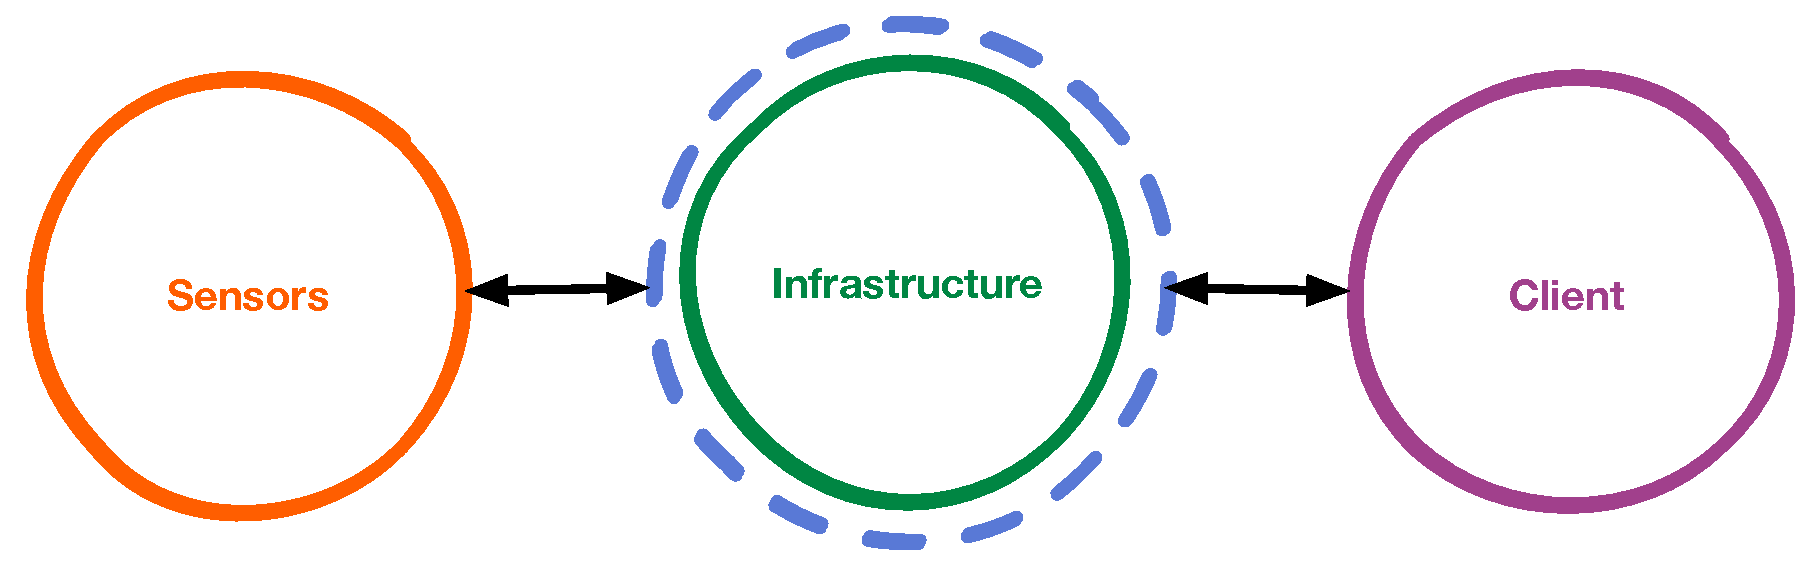
\includegraphics[width=\columnwidth]{figures/system_architecture.pdf}
  \caption{System architecture with communication layer. The dotted line shows the encapsulation in the REST and WebSocket layer.}
  \label{fig:architecture}
\end{figure}

\subsection{Sensors}
To gather data about the user's presence and availability we use sensors.
This project has been restricted to look at sensors that are available in commodity laptops.
We define a commodity laptop to be a device you can buy at any computer store.
The device should be able to run your operating system of choice.
It should have a camera, an input device, a microphone and radios such as Wi-Fi and Bluetooth built-in.

In this section, we will have a look at some of the sensing capabilities of a commodity laptop.
We will discuss the strengths and weaknesses of these sensors.
As well as providing, some reasoning for choosing the sensors we have used in our client.

\subsubsection{Keyboard and Mouse}
By using the mouse and keyboard as sensors, we collect every mouse movement and keyboard events and send the last recorded activity every second.
With this information, we can infer presence because there is someone triggering these events.

The issue with using keyboard and mouse as sensors is that even though they are a strong indicator of presence, we cannot decipher, based on these two sensors alone, who or what this presence is.
We can tie the machine to a specific user, but we cannot infer if a colleague is using the machine or if a cat decided to rest on the keyboard.

Another issue with mouse and keyboard sensors is that they provide a very weak indicator of non-presence.
When a key is pressed or the mouse moved, we know that someone is interacting with the machine, but the lack of action cannot tell us whether a user is present or non-present.
A user could be talking on the phone, reading, watching a video etc. all in which the user is present, but the mouse and keyboard cannot provide us with this information.

In terms of interruptibility, the information from the mouse and keyboard is too ambiguous to deduct whether a user is busy or interruptible.
Even If we knew the identity of the user sitting in front of the computer, it would still be difficult to determine whether the behavior is an indication of interruptibility.
An approach to determine interruptibility based on these sensors, would involve sending all information to the decision logic, effectively acting as a key logger, and therefore raising security and privacy issues.

\subsubsection{Microphone}
The use of a microphone as a sensor allows Approximator to sense the presence of a user, even if the user is not directly interacting with the machine.
With more advanced speech recognition, algorithms could identify the person(s) speaking.
This would provide us not only with presence, but also with identity, which was a problem with the keyboard and mouse sensors.

The same issue with the detection of non-presence also appears with the microphone, it is not possible to infer absence from the lack of sound.
As described with the keyboard and mouse sensors, a user can perform activities that does not trigger the sensor, and thus be present without detection.

Beside the detection of presence, the microphone provides a tool for inferring interruptibility.
According to Fogarty et al. \cite{fogarty2005predicting} speaking present a situation of non-interruptibility.

We have chosen to omit the microphone sensor.
There is a high risk of collecting too much noise compared to the signal we need.
The work environment would need to be very quiet for us to use a normal microphone as a reliable sensor.
For this reason, we have dropped the microphone sensor.

\subsubsection{Camera}
Like the microphone, the camera enables Approximator to sense the presence of a user without the user having to interact with the machine, but differs in the way it does so.
In the setting of a room, a microphone can sense if someone is in the room, but it is hard for the microphone to infer where in a room that they are located.

The camera can sense if someone is directly in front of the screen, which supplies a powerful indicator of presence, as well as an indicator of non-presence.
Unlike the other sensors, the camera can sense if a user is sitting in front of the machine, even if the user is not directly interacting with the machine.
However even though the camera can infer non-presence, there are still some issues.
If a user is located in their office but not visible to the camera, the sensor will infer this as absence.

The camera could apply face-recognition in order to determine the identity of the user present.
It could detect actions that the user is executing e.g. entering the room leaving, leaving the room, reading a book etc. that measures interruptibility.

\subsubsection{Bluetooth and Wi-Fi}
These radios can detect other devices such as mobile devices or beacons.
If we assume that, a user carries their mobile device with them, then the Bluetooth or Wi-Fi beacon from their device can be used to infer the users proximity to the machine.
Another usage is if the office the user works in have, beacons installed at the workplace, either as Bluetooth or Wi-Fi beacons, then the machine can infer its current symbolic location.
This can infer presence by detecting if the mobile device is nearby.
The issue here is if the user should forget their mobile device, either nearby the machine or at home.
In these cases the sensor would receive false data i.e. data that provides wrongful information regarding presence or interruptibility.
These sensors rely heavily on factors and devices external to the user's laptop, which makes it more volatile and prone to errors.

\subsubsection{Light}
The light sensor measures the ambient light of the environment.
This can sense if the laptop is in a dark or light room.
The deduced presence information from this sensor is redundant.
We already know that a user is present if they are using the mouse or keyboard. In addition, if they are visible on camera we know that they are present.
The camera can also detect the lighting level in a room, so the light sensor seems to be irrelevant.

\subsubsection{Process monitor}
This sensor is slightly different from the others since it primary purpose is not to sense presence, but interruptibility.
The idea of the process monitor is to supply it with a list of processes (programs) running on the user's computer that it should monitor.
This list consists both of work and leisure associated processes and the process monitor report if any and which program are in the foreground.
Through this, we obtain the same or weaker notion of presence and non-presence as we did with the keyboard and mouse sensor, but gain a stronger tool to infer interruptibility.

\subsubsection{Geo-location}
This sensor works by looking up the machines registered IP address, or if available uses the machines built-in GPS, and uses this to acquire a geographical address.
Knowing the whereabouts of the machine neither infers presence nor interruptibility on its own.
However, it does supply the other sensors and the decision module with useful information regarding the geographical setting of the machine.
The simplest use of this is to detect if the machine currently resides at the office, home, or another location.
Nevertheless, one of the more useful appliances would be in combination with the camera.
If the camera can detect action such as a user entering or leaving the room, this information could tell us whether the a user is in close proximity to the machine, but only that.
Combined with even the coarse location of the machine, Approximator could infer that a user was in a specific office, in close proximity the machine.

\subsubsection{Calendar Sensor}
This sensor can look at the user's calendar and get information about events entered here.
Events can help identify a user's activities during the day, like scheduled meetings or conference calls that would render the user non-interruptible.
Then we rely on the calendar data to be very accurate.
That is probably not always the case. For instance if a meeting is cancelled and the user does not update his calendar, the model would believe that the user was unavailable.
This uncertainty has excluded the calendar sensor in this first version of the project.

\subsubsection{Chosen Sensors}
The project scope limits us from using sensors outside of a commodity laptop and from using sensors, which require prior knowledge of the environment or the user.
This limitation excludes the calendar sensor, geo-location and the Process monitor, as they all require prior knowledge about the user.
The Calendar sensor needs to know which calendar provider the user is using, the Process monitor requires information on which program are work related for the user and Geo-location needs to know to which areas are home, work and otherwise.
We have excluded The Bluetooth and Wi-Fi sensors since they rely on external beacons to signal position.
The microphone would be a good choice as a sensor, but as most software developers work in shared offices this would generate a significant amount of noise data.
Therefore, we have chosen to omit the microphone.
By using the Camera, Keyboard and Mouse as sensors, we stay within the scope of the project, and still get a good amount of data to use in our interruptibility model.
By using the camera as sensor, we can omit the light sensor, due to redundancy in sensor features.

Our final choice of sensors are camera, keyboard and mouse.

\subsection{Infrastructure}
To provide presence and availability information to cloud workers we need a few things.
Firstly, we need to gather data input from the working environment.
Secondly, we need to aggregate this data and combine it for each user. Lastly we need to look at the data and through analyzes provide presence and availability information.

Our infrastructure handles the tasks. It can read input from sensors and analyze this with a decision module.
The workflow of the infrastructure is:

\begin{enumerate}
  \item Gather data.
  \item Aggregate data.
  \item Analyze data.
  \item Provide data.
\end{enumerate}

\subsubsection{Design}
The infrastructure supports multiple sensors for each user.
This modelling can lead to a very high amount of sensors connecting to the system.
To support this scalability need we base our system on the actor model by Carl Hewitt \cite{hewitt1973universal}.

Many software applications builds on the object oriented model.
The actor model is an alternative way to model computer programs.
In the actor model, the unit of work is an actor.
In object oriented programming the unit of work is an object.
Actors communicate by sending messages to each other.
Actors does not share state, making it possible to run actors in parallel and even on different machines.
This makes the actor model a good candidate for building highly scalable applications.

There are several frameworks implementing the actor model, such as Akka \cite{akka}, Project Orleans \cite{orleans} and most famously Erlang \cite{erlang}.
For this project, we have chosen Akka because it is Java based.
This supports the technical knowledge in our group.

We use the general programming language Scala \cite{scala} to program our Akka-based infrastructure.


\begin{figure}[H]
  \centering
  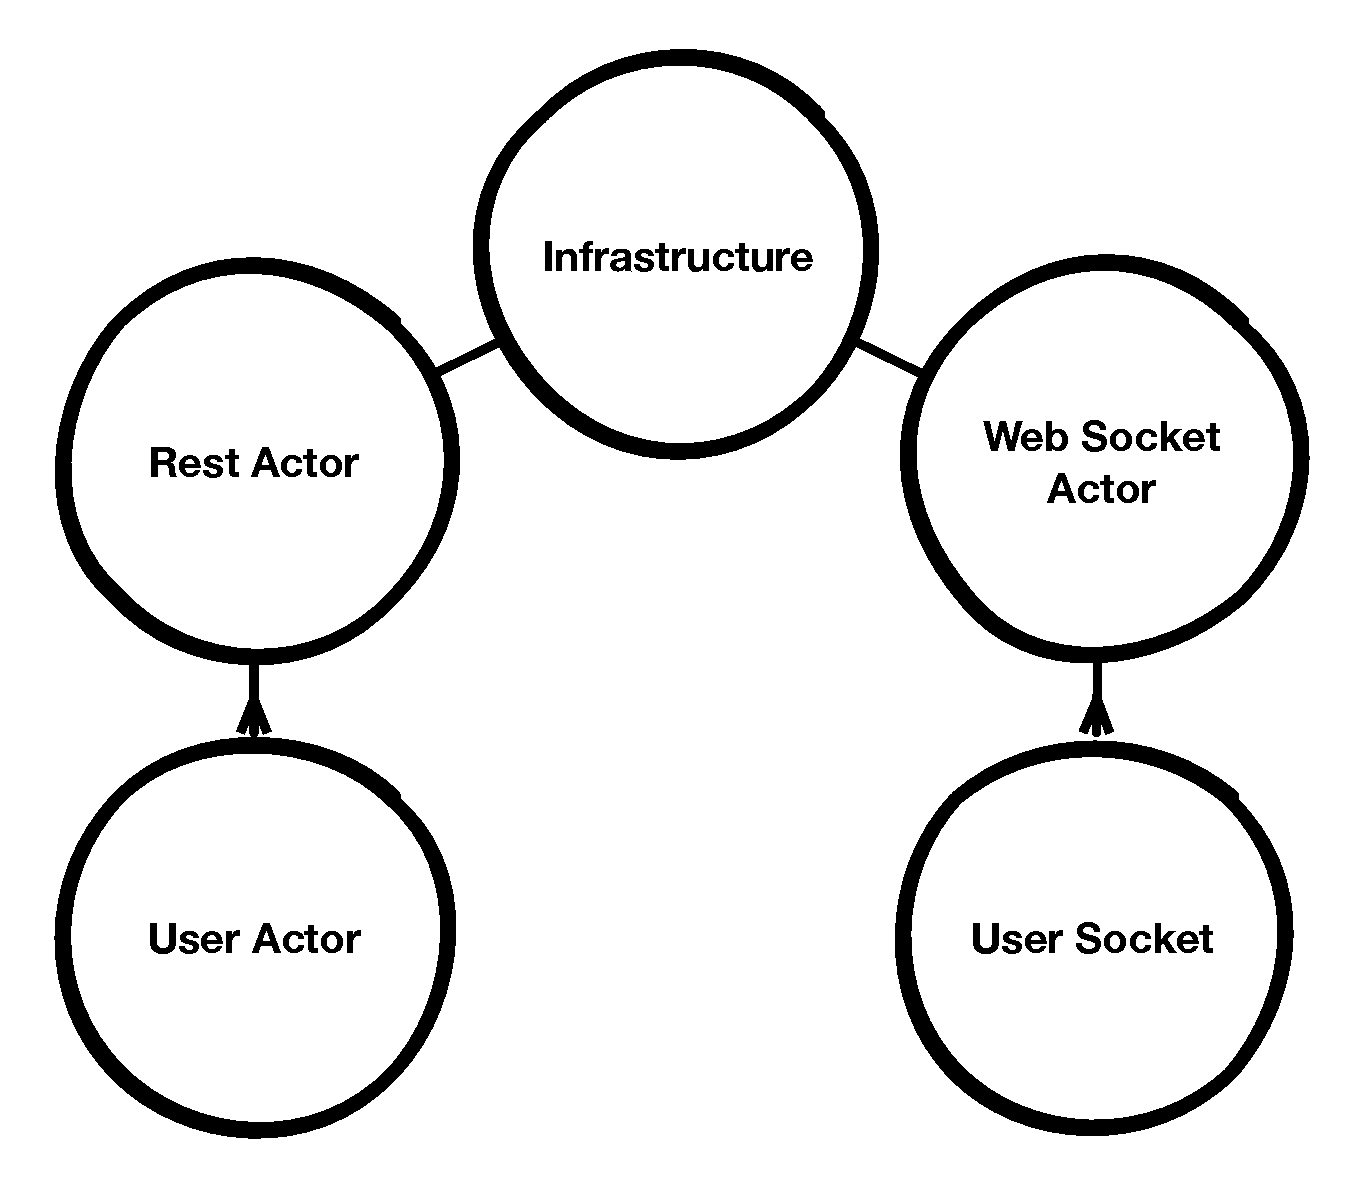
\includegraphics[width=\columnwidth]{figures/infrastructure_design.pdf}
  \caption{Infrastructure Design.}
  \label{fig:infrastructure}
\end{figure}

It is possible to deploy Akka applications on a server, which can run Java.
For this project, we have chosen to deploy our system to Azure \cite{azure}, Microsoft's cloud service for developers.
Having the infrastructure running at a cloud provider makes it reachable from the standard internet.
This enables us to build sensors and demonstrators that can run anywhere; as long as they have an internet connection, they can reach our infrastructure.

\subsubsection{Data}
Gathering data happens by sensors providing data.
To communicate with our infrastructure a sensor needs to register with the service.
When a sensor registers itself. it provides a username.
The username aggregates a group of sensors together around the notion of user.

\subsection{Client}
Windows based user installable application.
The sensor actually combines two parts of the system.
We have built the sensors into the client.
This enables ease of use for the end-user.
Merging the two parts makes it possible to get both parts on the user's laptop with a single installation.

\subsubsection{Ease of deployment}
We have focused on creating an easy to deploy system.
The infrastructure component deploys to any server capable of running the Java Virtual Machine (JVM).
Currently it is possible to get the source code, for the server as well as the client, from GitHub\footnote{\url{https://github.com/mofus/GSE}}.
The server source code requires Java and SBT.
With the source code on the server it is a simple run command, which will compile, fetch dependencies and run the infrastructure.

The client source code requires a .NET compiler.
The client is even easier since this is a normal Windows application.
The application is installable on any newer Windows installation.

The client's source code is available in our GitHub repository.
The client use the .NET framework, which makes it easy to build the client on other platforms with the Mono compiler.


\section{Decision Logic}
\label{sec:decision_logic}
We want to identify a software engineer's interruptibility value using the sensors in a laptop.
To achieve this there are three sensors providing data; keyboard, mouse and camera (face detection).

Raw sensor data does not say much about presence or availability.
We analyze the captured sensor data with a decision module in the infrastructure.
The decision module can calculate interruptibility values from the sensor inputs.

\subsection{Building a model}
We use a manual classification approach to classify the collected data.
We have recorded two test subjects, user A and user B in their work environment.
User A showed a clear coalition between patterns in the sensor data and the reported interruptibility.
We identified three major scenarios by looking at the data from user A; see  Figure~\ref{fig:scenarios}.

\begin{figure}[H]
  \centering
      \begin{tabular}{@{}llll@{}}
      \toprule
      \textbf{Scenario} & \textbf{1} & \textbf{2} & \textbf{3}      \\ \midrule
      Interruptible     & No         & No         & Yes             \\
      Primary sensor    & Camera     & Keyboard   & Mouse           \\
      Example task 1    & Reading    & Writing    & Browsing        \\
      Example task 2    & Video Chat & Coding     & Switching tasks \\ \bottomrule
      \end{tabular}
  \caption{The three identified scenarios.}
  \label{fig:scenarios}
\end{figure}

User B however did not show any clear indication of patterns that could identify a given scenario.
This could be because software engineers work in different ways.
There is also a chance that User B is an outlier and therefore not representing the generic software engineer.
Our problem is that we do not know.
It might as well be user A, who is the outlier.
It would have been much clearer if any of these theories were true if more test subjects had been involved.

\subsection{Scenario detection}
\label{scenario_detection}
We use a centralized algorithm to detect the user's scenario.
The algorithm is running on the infrastructure server.
Here it constantly looks at a moving window of incoming sensor data.
The window is 30 seconds long and contains all the sensor data from this period.
See the algorithm in Figure~\ref{fig:decision_logic}.

\begin{figure}[H]
  \centering
  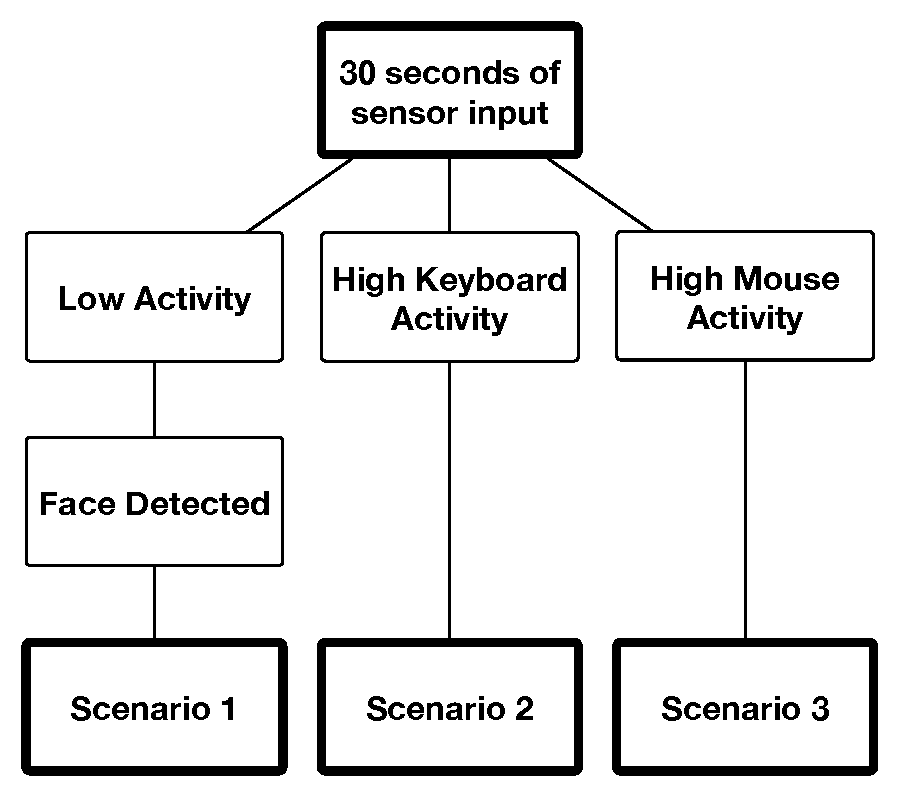
\includegraphics[width=\columnwidth]{figures/decision_logic.pdf}
  \caption{Decision logic for detecting scenarios.}
  \label{fig:decision_logic}
\end{figure}

\textbf{Scenario 1} is detected using face detection.
If a user is sitting in front of the computer, the face detection will detect the user as being present.
Detection happens with a frontal or profile detection depending on the angle the camera sees the users face.

We try to catch the scenario of a user sitting in front of the computer using it without the mouse and keyboard as main input.
This could be because the user is reading, having a conversation or something similar.

The keyboard sensor identifies \textbf{scenario 2}.
When a user is typing away, the user is doing concentrated work.
This work can be writing, coding or other keyboard heavy tasks.

When a user is moving the mouse a lot, we identify it as \textbf{scenario 3}.
We hypothesize that heavy mouse activity is an indicator for casual activity.
This could be browsing, moving files or simply a switch of context between work sessions.


\section{Evaluation}
In order to compare the performance of Approximator to the result from Forgarty's study, we follow the same method for evaluation during the experiments in this paper.

\subsection{Method}
\label{method}
Our experiment had two phases.
First, we did a video recording of the two test subjects in their work environment.

During the video recording Approximator was recording sensors data.
For the second phase, we did a survey to have humans assess the interruptibility of the video subjects.
We chose estimator subjects from the software development community.
The participants assessed the interruptibility based on short sequences of video, showing the video subjects in random selected situations in their work environment.

\subsubsection{Stage One}
The two male video subjects were 25 and 34 years of age.
The first video subject worked for a security company where his primary task was to maintain and develop on the company system.
Since the company also have offices in other countries, this video subject often did parallel development with the out-of-country teams.
He worked in shared offices, where he shared the office with 3-4 other employees, often people assigned to the same project or with a similar skillset.
It was possible to close the door to these offices, but that rarely occurred.

The second video subject worked for a software company where his primary task was to develop server solutions.
The company has offices in several locations, including home offices.
Our video subject worked in a home office, placed in the basement of his house.
Either all communication with colleges happens online, through instant messaging or audio chats.

A Sony Handycam HDR-CX360 with a wide-angle lens recorded the videos.
The video format was mp4 with a resolution of 720x576 at 25 frames per second.
The recording was with sound, but we removed the sound before the survey.
We did this because Approximator does not use the microphone, so we deemed it unfair if the estimator subjects had this extra information.
The camera angle did not allow for the content of their screen to be visible.
The angle did however show as much of the office as possible, while showing the face of the video subject.

\begin{figure}
  \centering
  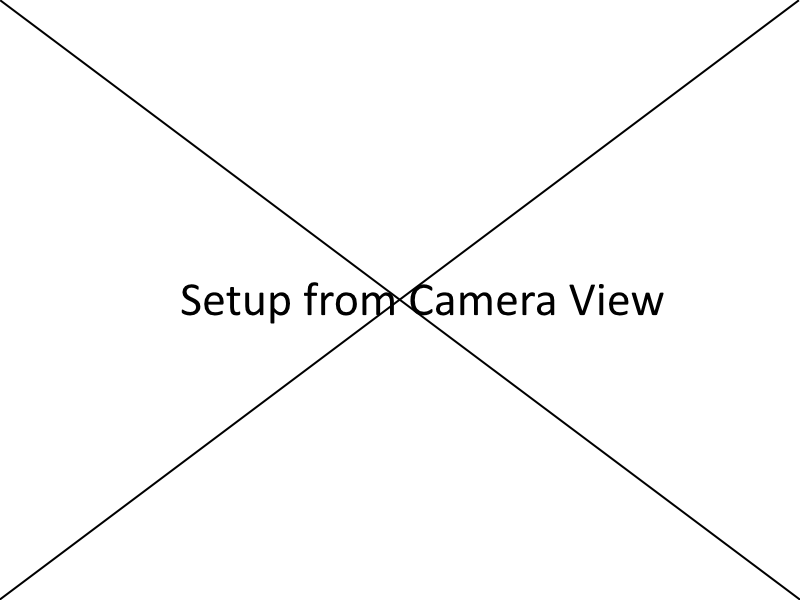
\includegraphics[width=\columnwidth]{figures/experiment_setup.png}
  \caption{View of experiment setup.}
  \label{fig:experiment}
\end{figure}

Approximator was running on a Microsoft Surface Pro 3 i5 processer 8GB Ram with Windows 8.1 OS (user a).
And a Lenovo T440s Intel Core i5 64-bit processer 8GB RAM with a Windows 7 OS (user b).
Both machines mounted in an office dock setup connecting the machine to an external screen, keyboard and mouse.
Approximator utilized the keyboard, mouse and camera as sensors, and sent data from these sensors to the infrastructure throughout the experiment.
The video subject got a visual and audible prompt at random intervals averaging at two times per hour.
At each prompt the video subjects self-reported their own level of interruptibility on a scale of one (highly interruptible) to five (highly non-interruptible) by show of fingers on one hand when prompted.
The video subjects had no way of pausing the application, but could request retroactively to have sequence deleted if necessary.
We removed the recordings where the video subjects was not present during a prompt.
If it should happen that the video subjects clearly registered the prompt, but did not signal their interruptibility, due to them being on the phone or engaged in another activity that required their full attention, then we would interpret these as highly non-interruptible events.

The experiment spanned two workdays from 9 am to 4:30 pm, yielding a total of 30 hours of video and 43 prompts.

\subsubsection{Stage Two}
\label{stage_two}
At this stage, we created an application with the explicit purpose of peer reviewing the collected data.
We chose estimator subjects from the software development community to partake in the survey under supervision from two of the researchers.

When the estimator subjects started the survey, they were asked to rate each video on a scale of one (highly interruptible) to five (highly non-interruptible).
Estimators should act as though they were colleges with the video subject.
They should ask the researchers if they had any questions before they started the survey.
Afterwards they were required to enter their demographic information.
These demographical questions consisted of gender, age, and ethnicity.
The demographic distribution may affect people's ability to interpret interruptibility.

\begin{figure}
  \centering
  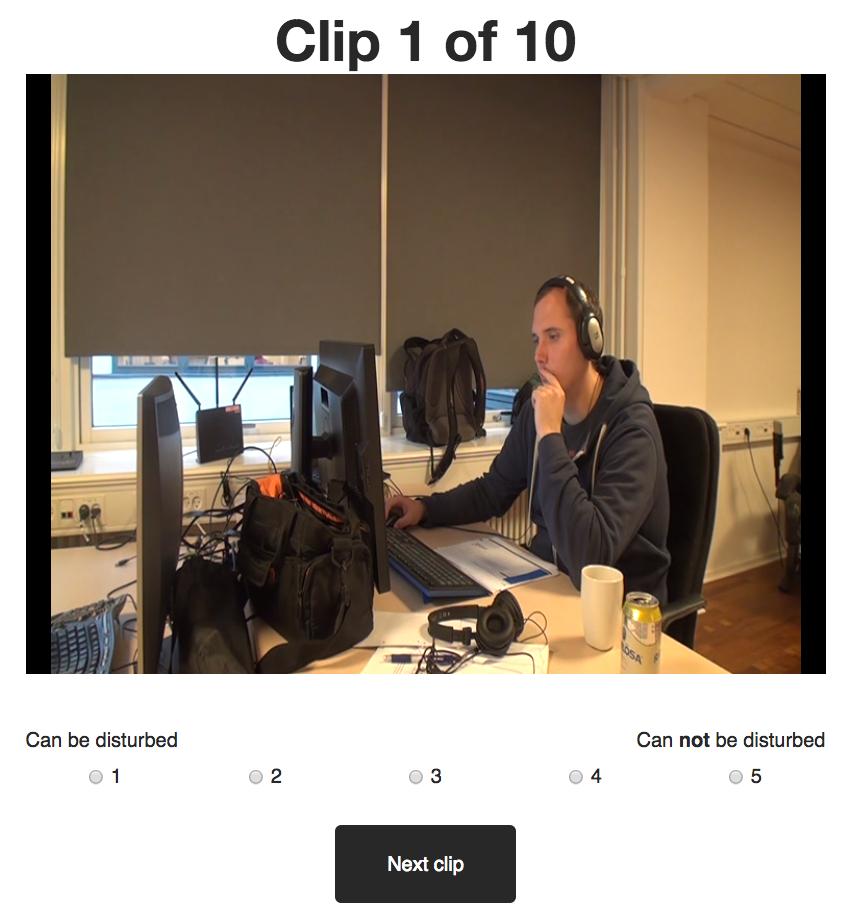
\includegraphics[width=\columnwidth]{figures/webpage_screenshot.png}
  \caption{Screenshot of survey webpage.}
  \label{fig:webpage}
\end{figure}

The content survey consists of five unique sets with seven different video clips from the first stage of the experiment.

Each clip contained the last 30 seconds leading up to the video subjects prompt for self-reporting.

Each estimator subject saw one of the five different sets of video with three random repetitions from the same set.
The three random repetition is to ensure that the estimator is confident about their answer.
If more than two repetitions deviated more than two points compared to the original answer, the results from that estimator subject was invalid.
The estimator could replay the sequence as many times as they wanted until they felt they could give a valid assessment.
Each sequence played in full length before the user could rate it and proceed to the next.

\subsection{Data analysis}
After the experiment concluded, we compared the data from Approximator to the data from the survey by plotting the values into two confusion matrices.
One comparing the answers of video subjects to answers of the estimator subjects.
Another comparing the answers of the video subjects to the results of Approximator.
By finding correlations between hits in the video / estimator and video / Approximator results, we could compare how Approximator performs in relation to human judgment, while also comparing our findings to those found by Fogarty et al. \cite{fogarty2005predicting}

\subsection{Results}
In this section, we will go over our results that we have collected through the experiments mentioned in \nameref{method}.
This section contains the results collected from the review group and the results collected from Approximator.

\subsubsection{Review Group Results}
Out of the 43 prompts, we used 35 for the review test.
The remaining eight was not applicable since the test subject was not present at the time of the prompt.

\begin{table}[h]
  \centering
    \begin{tabular}{@{}llllll@{}}
    \toprule
    \textbf{Interruptibility} & 1 & 2 & 3 & 4 & 5  \\ \midrule
    \textbf{Frequency}        & 9 & 6 & 3 & 9 & 8  \\ \midrule
    Total number of prompts   &   &   &   &   & 35
    \end{tabular}
    \caption{Frequency of interruptibility values reported by the test subjects, ranging from 1 (highly interruptible) to 5 (highly non-interruptible).}
    \label{fig:interruptibilityFrequency}
\end{table}

19 volunteers chose to participate in the survey.
Four volunteers surveyed the video clip sets A, B, C and D while three volunteers surveyed set E.
All surveys were valid and consistent answers.

Although answers were consistent and the volunteers clearly understood the task, the accuracy of the volunteers were overall poor.
As shown in \autoref{tab:survey_accuracy} the average precision among all sets were around 28\%.
We attribute this low score to the fact that is very hard to precisely rate another person's interruptibility on a scale from one to five.
In order to account for this we use the same scale conversion as Fogarty\cite{fogarty2005predicting}.
However, unlike Fogarty who did the scale conversion, by converting all values from 1-4 as 1 and 5 as 5, we did it as follows. For all answers in the survey, we changed values of 1-3 to be 1 and 4-5 to be 5.
This gave us a binary representation of interpretation of the data.
As shown in \autoref{tab:survey_accuracy} that yielded a much improved average accuracy of 63\%.
The reason that we converted the data differently from Fogarty lies in Forgarty's reason for converting the data in the first place.
Forgarty's data showed that the estimator subjects had a tendency to rate the video subjects' interruptibility lower than the self-reported value.
Our data shows that there is an even distribution between lower and higher rated values.

During the data acquisition, we compared the result from the review group to the results from the video experiment.
See a confusion matrix in \autoref{fig:video_to_estimator_matrix}.
Rows correspond to the values reported by the video subjects, and columns correspond to the values from the estimator subjects.
The unshaded diagonal represents instances when the estimator subject correctly estimated the same value given by the video subject.
This matrix shows that the overall accuracy lies at 30.08\%, and the accuracy within one is at 62.41\%.
This shows that our review group was about as accurate as Forgarty's review group \cite{fogarty2005predicting} that achieved an overall accuracy of 30.7\% and a within one accuracy of 65.8\%.

As discussed in \nameref{stage_two} the demography of the participants could have impact the interpreted interruptibility of other people.
\autoref{fig:demography} shows the distribution of participants by country of origin, age and gender.

%Estimator comparison
\begin{figure}[h]
  \centering
  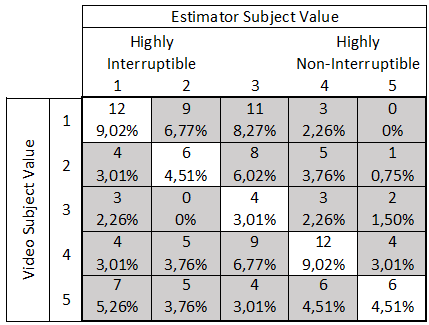
\includegraphics[width=\columnwidth]{figures/VideoToEstimatorConfusionMatrix.png}
  \caption{Confusion matrix comparing the estimator subject values to the values of the video subject. \\Overall Accuracy: 30.08\% Accuracy within 1: 62.41\%}
  \label{fig:video_to_estimator_matrix}
\end{figure}

\begin{figure}[h]
  \centering
  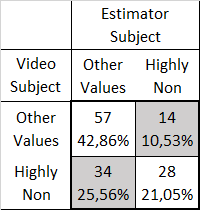
\includegraphics[width=\columnwidth/2]{figures/VideoToEstimatorReducedConfusionMatrix.png}
  \caption{Reduced confusion matrix comparing the estimator subject values to the values of the video subject. \\Overall Accuracy: 63.91\%}
  \label{fig:reduced_video_to_estimator_matrix}
\end{figure}

\subsubsection{Approximator Results}
The sensors from Approximator collected data throughout the 30 hours of the experiment resulting in a total collection of 86823 mouse events, 16151 face detection events and 28629 keyboard events.
In our experiment, we only took the events into account that could be compared to the video subjects' self-reports.
This was the data collected during the videos used in the survey. See the distribution of these events in \autoref{tab:event_distribution}.
\autoref{fig:video_to_approximator_matrix} contains a comparison of the data produced by Approximator with the values reported by the video subjects.

\begin{table}[h]
  \centering
  \begin{tabular}{@{}lll@{}}
    \toprule
     & Video subject 1 & Video subject 2\\ \midrule
    Mouse events       & 984    & 534    \\
    Keyboard events       & 319    & 218    \\
    Face detection events       & 244    & 113    \\ \midrule
    Total   & 1547 & 865\\ \bottomrule
  \end{tabular}
  \caption{Distribution of events collected by Approximator divided over the Video subjects}
  \label{tab:event_distribution}
\end{table}

The overall accuracy of Approximator was 31.43\% making it slightly more accurate than the estimator subjects assessments by 1.35\%.
When we looked at the reduced matrices \autoref{fig:reduced_video_to_estimator_matrix} and \autoref{fig:reduced_video_to_approximator_matrix}, we saw that the overall accuracy from the estimators were 1.05\% better than Approximator's accuracy.
This seemed odd to us, so we took a closer look at the interruptibility values produced by Approximator.
The investigation showed that video subject 2 values was very accurate with an overall accuracy of 41.67\% with a within one accuracy of 91.67\%.
However, the investigation also showed that the values for video subject 1 was all ones (highly non-interruptible).

The reason for this strange abnormality has five possible reasons.
\begin{enumerate}
  \item The readings are correct, and video subject 1 was prompted when at interruptibility value 1.
  \item Video subject 1 did not do much work during the 2 days of recording, but did not want that to appear on the results.
  \item The sensor units were in some way faulty.
  \item The decision module was in some way faulty.
  \item The decision module's interruptibility model does not recognize video subject 1 work patterns.
\end{enumerate}

We can exclude 1 due to the self-report stating otherwise.
Reason 2 seems unlikely due to review groups assessment was more accurate on video subject 1 than on video subject 2.
\autoref{tab:event_distribution} shows that there is plenty of sensor input on all sensor channels which can excludes reason 3.
Reason 4 is also unlikely since the same module processed the data of both video subject 1 and 2.
Reason 5 is the most likely since the interruptibility model, \autoref{fig:scenarios} relies heavy on keyboard input to infer non-interruptibility and mouse events to infer interruptibility.
\autoref{tab:event_distribution} shows that that video subject 1 have an approximately 1:3 ratio of keyboard vs mouse events, whereas video subject 2 have an approximately 1:2 ratio of keyboard vs mouse events.
This gives an indication that video subject 1 work tasks are more mouse based than those of video subject 2.
This leads to Reason 5 being the conclusion because the interruptibility model described in section \nameref{scenario_detection} infers that heavy mouse activity is an indicator for casual activity, which does not seem to be the case.

%Approximator comparison
\begin{figure}[h]
  \centering
  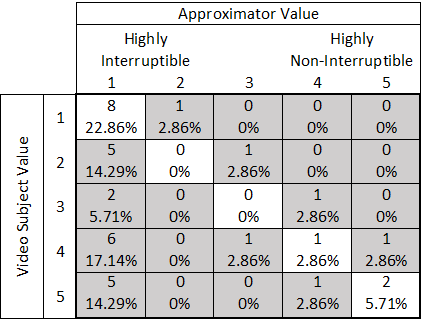
\includegraphics[width=\columnwidth]{figures/VideoToApproximatorConfusionMatrix.png}
  \caption{Confusion matrix comparing the values produced by Approximator to the values of the video subject. \\Overall Accuracy: 31.43\% Accuracy within 1: 62.86\%}
  \label{fig:video_to_approximator_matrix}
\end{figure}

\begin{figure}[h]
  \centering
  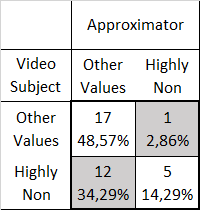
\includegraphics[width=\columnwidth/2]{figures/VideoToApproximatorReducedConfusionMatrix.png}
  \caption{Reduced confusion matrix comparing the values produced by Approximator to the values of the video subject. \\Overall Accuracy: 62.86\%}
  \label{fig:reduced_video_to_approximator_matrix}
\end{figure}

%Anders data only
\begin{figure}[h]
  \centering
  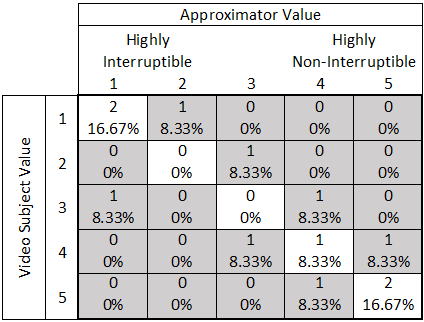
\includegraphics[width=\columnwidth]{figures/VideoToApproximatorConfusionMatrix(AndersValues).png}
  \caption{Confusion matrix comparing a subset of values produced by Approximator to the values of the video subject. \\Overall Accuracy: 41.67\% Accuracy within 1: 91.67\%}
  \label{fig:subset_video_to_approximator_matrix}
\end{figure}

\begin{table}[h]
  \centering
  \begin{tabular}{@{}lll@{}}
    \toprule
    Test Set     & Adjusted & Original \\ \midrule
    A       & 50.99\%    & 21.42\%    \\
    B       & 57.14\%    & 21.42\%    \\
    C       & 82.14\%    & 39.28\%    \\
    D       & 78.57\%    & 32.14\%    \\
    E       & 47.61\%    & 28.57\%    \\ \midrule
    Average & 63.09\%    & 28.57\%    \\ \bottomrule
  \end{tabular}
  \caption{Accuracy of survey participants interpreting test subjects interruptibility}
  \label{tab:survey_accuracy}
\end{table}

\begin{table}[h]
  \centering
    \begin{tabular}{@{}llllll@{}}
    \toprule
    \textbf{Country}        & count & \textbf{Age} & count & \textbf{Gender} & count \\ \midrule
    Denmark                 & 13    & 18-24        & 7     & Male            & 16    \\
    Romania                 & 3     & 25-34        & 10    & Female          & 3     \\
    Belgium                 & 1     & 35-44        & 1     &                 &       \\
    Germany                 & 1     & 45-54        & 1     &                 &       \\
    Poland                  & 1     &              &       &                 &       \\
    Total participants      & 19    &              & 19    &                 & 19    \\ \bottomrule
    \end{tabular}
    \caption{Demography of survey participants by Country of origin, age and gender.}
    \label{fig:demography}
\end{table}

\section{Discussion}
Many factors affect how people assess human interruptibility as noted in \cite{Avrahami2007}.
These aspects are hard to incorporate in prediction models.
In this paper, we use a limited demography of people to assess interruptibility.
Factors like culture, age and ethnicity may significantly influence the results.

This paper bases its research background and evaluation of the work done in \cite{fogarty2005predicting} but has a number of different factors.
Over 10 years has passed since \cite{fogarty2005predicting} was written.
Moreover, whereas \cite{fogarty2005predicting} relied heavily on factors like closed office doors and talking on the phone.
Today open office spaces with are much more common than in 2003 and talking on the phone is less common in favor of other means of communication like email, and chat.
More notably \cite{fogarty2005predicting} based their studies on knowledge workers in a University administration department while we base our paper on software developers in a CSCW setting.

We had hoped that both our test subjects would show the same coalition in their data.
This was unfortunately not the case.
If a similar project is to succeed, we need a better algorithm for detecting patterns.
Instead of having a centralized generic algorithm, we could have learning algorithms on each users' machine.
An algorithm which could be tailored directly at a given users' needs would be preferable.
One approach is to construct an algorithm with a learning period.
In the learning period, the user needs to answer interruptibility questions at random intervals.
This way the algorithm could build up some training data to use for future evaluations.

The current sensors only give vague clues to a person's context, through the level of activity.
Additional sensors that could give input about the context, especially in combination with a learning algorithm, could improve our results.
Sensors that could give specific clues to the context about how a subject was working e.g. advanced gaze tracking, speech detection, posture detection, desktop monitor, process monitor etc..
Sensors like these would allow for more detailed and less ambiguous interruptibility models, and thereby better accuracy.

\subsection{Future Work}
We chose to focus our paper on the sensors available in a modern laptop for the ease of use and ease of deployment.
Most people today also carry smartphones and newer devices such as fitness trackers and smartwatches are gaining popularity.
These devices could supply additional useful data to our infrastructure to enhance the modeling of interruptibility by providing more fine-grained position and movement.

\section{Conclusion}
We set out believing that it was possible to detect a software engineer's interruptibility value using only the sensors in a laptop.
It turned out that it was possible for one of our two test subjects.
This finding opens more questions than it answers. Is our approach still valid have we tested on more subjects?

We conclude that our initial idea is valid.
However, our project did not include enough test subjects to say anything definite about the feasibility across all software engineers.

\section{Acknowledgements}
We would like to thank Paolo Tell for supervising and guiding us throughout the project.
We are also grateful for the great feedback from Thomas Olof Pederson and Shahram Jalaliniya.
Lastly, we would like to thank all the people who helped do our evaluation.

\balance
\bibliographystyle{acm-sigchi}
\bibliography{ubicomp}

\end{document}
